\section{Results}
% Without SOT:
% TM: (91.3 + 81.7 + 89.8 + 85 + 90)/5 = 87.56
% SP: (69.5 + 56.4 + 58.7 + 61.6 + 61.4)/5 = 61.52
\textbf{General Benchmark.} Table \ref{tab:tuned-benchmark} displays experiment results, showcasing models' performance with and without the SOT module. 
Without the SOT module, models achieve an average accuracy of 87\% on the \texttt{TM} dataset and 61\% on the \texttt{SP} dataset, 
demonstrating their capability to learn from limited samples. Notably, \texttt{B} stands out as the top performer across both datasets, 
while \texttt{B++} ranks the lowest among all methods.

% With SOT:
% TM: (86.4 + 81.9 + 87.1 + 89.6 + 89.1)/5 = 86.42
% SP: (55.8 + 65.8 + 64.9 + 68 + 66.4)/5 = 64.58
With the SOT module, models maintain an average accuracy of 86\% on the \texttt{TM} dataset, 
suggesting that the SOT module has minimal impact on performance. However, on the \texttt{SP} dataset, 
models exhibit an average accuracy of 65\%, marking a 4\% improvement.

Interestingly, the introduction of the SOT module causes a decline in \texttt{B}'s performance, 
while \texttt{MT} emerges as the top performer on both datasets with the SOT module. 
In summary, the best performance on the \texttt{TM} dataset is achieved by \texttt{B} without the SOT module, while on the \texttt{SP} dataset, 
\texttt{MT} with the SOT module leads. However, the differences in performance are marginal in both cases.


\begin{table}[ht]
\caption{
    \textbf{Benchmark Results.} Test accuracy of all methods on \texttt{TM} and \texttt{SP} in the 5-way-5-shot setting. We depict the average accuracy and the 95\% confidence interval both without (left) and with SOT (right) and the difference.
    \vspace{5pt}
}

\label{tab:tuned-benchmark}
\centering
\begin{tabular}{llllr}
\toprule
 &  & \multicolumn{2}{@{}c}{\textbf{Test Acc. (\%)}} & \\
 &  & w/o SOT & w/ SOT & Diff \\
\midrule
\multirow[c]{5}{*}{\texttt{TM}} & B & $90.7 \pm 0.7$ & $86.3 \pm 0.9$ & {\color{red} +4.8} \\
 & B++ & $81.9 \pm 0.9$ & $82.8 \pm 0.9$ &  {\color{teal} +1.1} \\
 & MAML & $\mathbf{92.8} \pm 0.5$ & $99.2 \pm 0.1$ & {\color{teal} +6.9} \\
 & MN & $84.6 \pm 0.8$ & $\mathbf{99.7} \pm 0.1$ &  {\color{teal} +17.9} \\
 & PN & $87.1 \pm 0.8$ & $98.6 \pm 0.2$ & {\color{teal} +13.2} \\
\midrule
\multirow[c]{5}{*}{\texttt{SP}} & B & $\mathbf{69.2} \pm 0.7$ & $55.7 \pm 0.8$ & {\color{red} -19.6} \\
 & B++ & $64.1 \pm 0.7$ & $64.6 \pm 0.7$ & {\color{teal} +0.8} \\
 & MAML & $68.7 \pm 0.7$ & $98.0 \pm 0.2$ & {\color{teal} +42.8} \\
 & MN & $68.2 \pm 0.8$ & $\mathbf{99.8} \pm 0.1$ & {\color{teal} +46.5} \\
 & PN & $63.5 \pm 0.7$ & $99.2 \pm 0.1$ & {\color{teal} +56.1} \\
\bottomrule
\end{tabular}
\end{table}
% \caption{
%     \textbf{Benchmark Results.} Test accuracy of all methods on \texttt{TM} and \texttt{SP} in the 5-way-5-shot setting. We depict the average accuracy and the 95\% confidence interval both without (left) and with SOT (right) and the difference.
%     \vspace{5pt}
% }

\textbf{Way-Shot Analysis.} Figure \ref{fig:way-shot} presents the way-shot analysis results for \texttt{PN} on the \texttt{TM} dataset, with and without the SOT module. 
The left subplot shows test accuracy against the number of classes, and the right subplot against the number of samples per class.

Without the SOT module, there's a predictable trend: accuracy decreases with more classes but increases with additional samples per class. 
% However, this pattern changes with the SOT module. Here, accuracy remains stable regardless of the number of ways or shots. Remarkably, in challenging scenarios like 10-way-1-shot, 
% the model sustains a high test accuracy of around 97\%.

\begin{figure}[h!]
    \centering
    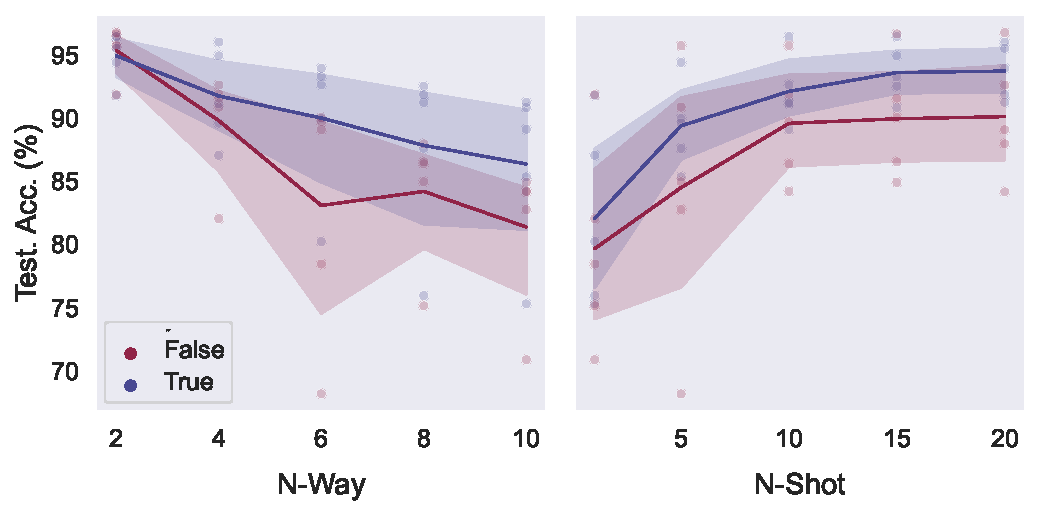
\includegraphics[width=1\columnwidth]{figures/way-shot.pdf}
    \caption{\textbf{Way-Shot Analysis.} Test accuracy of \texttt{PN} on the \texttt{TM} dataset with and without the SOT module in various 
    few-shot learning settings for fixed n-way (left) and n-shot (right). Individual points represent a single experiment. We show the regression line with a 
    95\% confidence interval.}
    \label{fig:way-shot}
\end{figure}
